\chapter{The CLI-Tutor Tool}
% - Tool (CLI-Tutor)
%   - overview
%       - curriculum
%       - lesson design
%            - deliberate emphasis on  easy vocabulary
%            - running examples
%            - refresher from previous lesson
%       - usability considerations
%       - safety considerations
%       - vocab and validation
%   - web version
%
\label{chap:clitutor}

\begin{lstlisting}[float=htbp, keepspaces, frame=single, language={}, label=lst:clihelp, caption=Output of the help flag of \textit{CLI-Tutor} running in a docker container.]
cli-student@3bc86f9090f9:~/tutor$ cli-tutor -h

        _ _       __        __
  _____/ (_)     / /___  __/ /_____  _____
 / ___/ / /_____/ __/ / / / __/ __ \/ ___/
/ /__/ / /_____/ /_/ /_/ / /_/ /_/ / /
\___/_/_/      \__/\__,_/\__/\____/_/

A simple command line tutor application that aims to introduce users to the
    basics of command line interaction.
    Web version is available at https://clitutor.chistole.ch

Usage:
  cli-tutor [flags]
  cli-tutor [command]

Available Commands:
  completion  Generate the autocompletion script for the specified shell
  help        Help about any command
  info        Prints information about the tool and log collection
  repo        Prints a url to the git repository for this tool
  version     Print the version number of cli-tutor

Flags:
  -h, --help            help for cli-tutor
  -n, --no-upload-log   Do not send a copy of the log to the developer
  -x, --no-welcome      Do not show welcome message when entering tutor

Use "cli-tutor [command] --help" for more information about a command.
\end{lstlisting}


\textit{CLI-Tutor} is a command line application written in the Go
programming language. It is an interactive tutorial focused on introducing
novices to the Linux command line environment. The application is intended to
be a forgiving but faithful representation of a shell running
\textit{Bash}\footnote{\textit{Bourne Again SHell}:
\url{https://www.gnu.org/software/bash/}}. In this chapter, we will discuss the non-technical design considerations and choices made during the development of \textit{CLI-Tutor}.

\section{Overview}
\subsection{Curriculum}

\textit{CLI-Tutor} is intended to be used with zero prerequisite knowledge of
the command line. To achieve this low barrier to entry, lessons are designed
from the perspective of catering to a complete novice user. The curriculum
consists of lessons that introduce the very basics of textual interaction and
shell usage. As of writing, \textit{CLI-Tutor} has 5 full lessons implemented
as a proof of concept and serve as the curriculum in the user study conducted
in this thesis work. \textit{CLI-Tutor} is designed to be easily extensible
with new lessons being easy to contribute. How this is achieved will be
discussed later in \autoref{chap:design}.

\subsubsection{List of implemented lessons} 

\paragraph{Basics of Textual Interaction.} This lesson covers the very
foundational concepts of textual interaction. The user is introduced to the
term \textit{CLI} and explained what a \textit{shell} is using an ASCII
graphic. The user is then introduced to the concept of issuing a command. To
sow interest, the user is then asked to execute some commands to illustrate that
the terminal is really interacting with their operating system. The Users are
asked to use the \textit{curl} from command to pull down a weather report from
the \url{wttr.in} as an example of what is possible with the command line.
Furthermore, the user is introduced to some important in-built commands
of \textit{CLI-Tutor} and taught how to clear the screen. Another feature
introduced to the user is \textit{zen-mode}, a feature that prevents the screen
from being cluttered with output of previous commands to prevent the user from
getting overwhelmed. This feature is activated by default in lesson 1 but is
then deactivated, unless explicitly set, for the remainder of the curriculum.

\paragraph{Getting more familiar with the shell.} This lesson jumps deeper into
the concept of issuing commands and the "grammar" behind a command. To make
this more intuitive the metaphor of a sentence is used, adapted from the
documentation of the \textit{cobra} command line tool
library\cite{franciacobra}. The lesson introduces users to fundamental concepts
such as sub-commands and flags. The user is then asked to perform a series of
tasks involving the \textit{wc} word counting core utility. These actions are
performed on a sample file that \textit{CLI-Tutor} creates and serves as a
running example throughout the tutor.

\paragraph{Basics of the file system and practicing commands.} Lesson 3 is all
about the file system. The file system and file system operations. The user is
first introduced to the prompt and given an explanation of all the different
sections of the prompt line. The prompt in \textit{CLI-Tutor} is modeled after
the stock prompt of many popular Linux distributions (see:
\autoref{lst:clihelp}, line 1), consisting of a username, hostname and current
working directory path. The user is introduced to the idea of a hierarchical
tree-like file system and is taught how to navigate around it. The \textit{ls}
command is also discussed and used to illustrate the concept of hidden files.
\textit{CLI-Tutor} also includes a hidden file that it places in the directory
the tutor is launched from to help illustrate the concept of hidden files. All
the example files included in lessons are deleted upon exiting the tutor. The
lesson closes with a long example for the user to try out that includes all the
concepts discussed in the lesson.

\paragraph{Shell shortcuts and tricks.} This lesson is aimed to be a bit more
fun and introduces the user to some tricks and shortcuts available in the shell
and the \textit{readline}\cite{ramey_fox_readline} library used for input in a
\textit{bash} shell environment. The user is introduced to the concept of a
shell history file and also of the reverse history search feature with
\textit{Ctrl+r}. The cancel \textit{Ctrl+c} command is introduced as well
as the \textit{!!} operator. As a final step, tab completion is introduced.

\paragraph{Helping yourself.} This is the last lesson of the current version of
\textit{CLI-Tutor} and covers how a user can go about seeking help at the
command line and helping themselves. The concept of pagers and some important
keybindings of the \textit{less} pager program are first explained before
introducing the \textit{man} command to the user. Users are also taught about
help flags and encouraged to check out the help command of \textit{CLI-Tutor},
shown at the very beginning of this \hyperref[chap:clitutor]{chapter} (see:
\autoref{lst:clihelp}).

\subsection{Lesson Design}
\subsection{Usability Considerations}
\subsection{Safety Considerations}
\section{Web Version}


\begin{figure}[htbp]
    \centering
    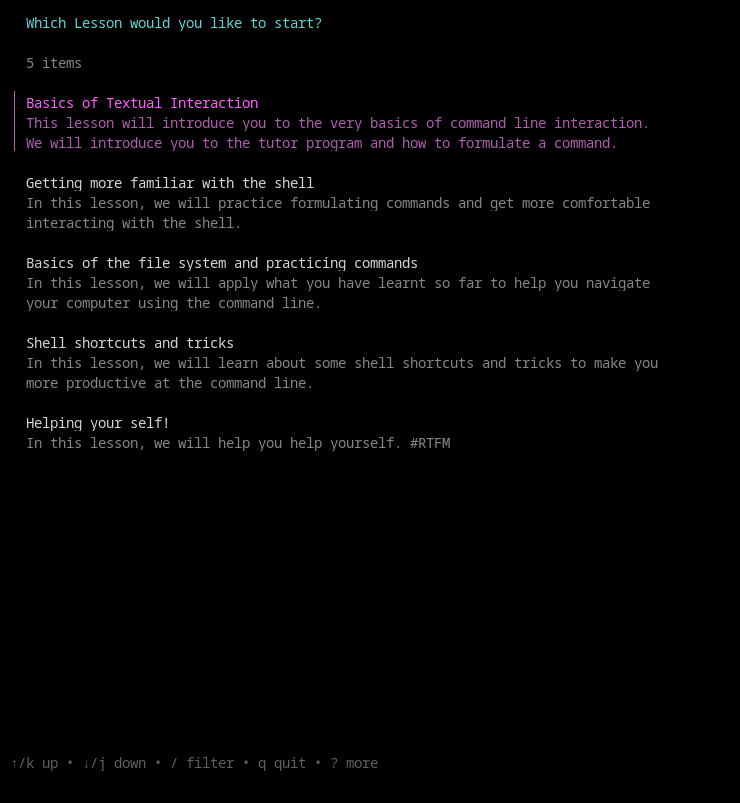
\includegraphics[width=0.8\textwidth]{img/climenu}
    \caption{Screen shot of \textit{CLI-Tutor} menu screen.}
    \label{fig:clitutormenu}
\end{figure}
\begin{figure}[htbp]
	\centering
	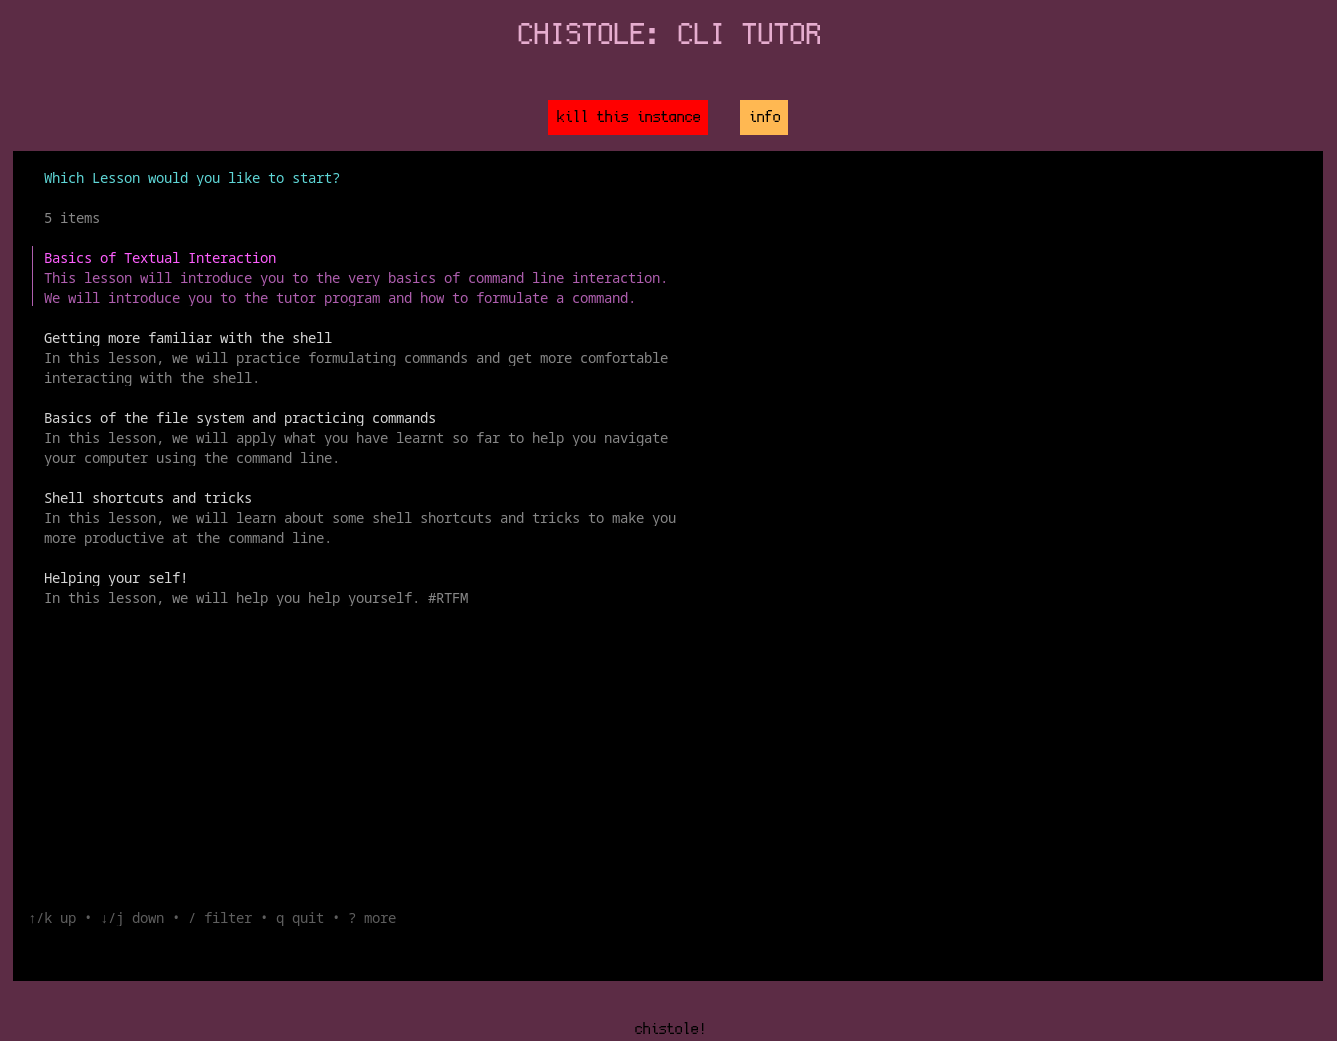
\includegraphics[width=1\textwidth]{img/cliwebfull}
	\caption{Screen shot of \textit{CLI-Tutor} menu screen in the web version.}
	\label{fig:webversion}
\end{figure}

\begin{figure}[htbp]
	\centering
	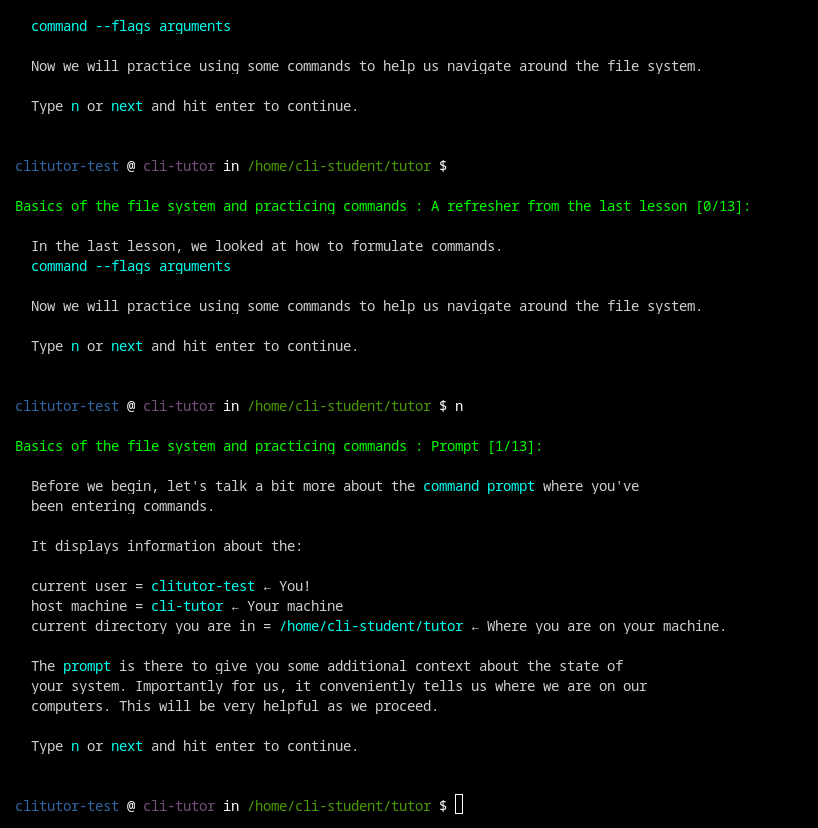
\includegraphics[width=1\textwidth]{img/cliexpansionfull}
	\caption{Screen shot of a \textit{CLI-Tutor} lesson showing values interpolated into the lesson.}
	\label{fig:webversion}
\end{figure}


